\section{Base Teórica}

La planificación es un componente fundamental del sistema operativo que se encarga de asignar tiempo de procesamiento a los diferentes hilos y procesos que se ejecutan en un sistema. En este capítulo se presentará la información necesaria para comprender la planificación a corto plazo, con un enfoque específico en el sistema operativo FreeBSD y su planificador 4BSD. Se describirán los conceptos fundamentales de procesos e hilos, incluyendo su estructura y estados, y se explicará cómo el planificador toma decisiones sobre cuál hilo o proceso debe ejecutarse en un momento dado. Además, se examinarán en detalle las operaciones de cambio de contexto, encolado, elección del procesador y remoción de hilos de la cola, que son funciones clave del planificador 4BSD. Con esta base teórica, se sentarán las bases para entender cómo funciona el planificador de FreeBSD y cómo puede ser mejorado.


\subsection{Procesos e hilos}

En sistemas operativos, los procesos son entidades aisladas que representan la ejecución de una tarea o aplicación en particular. Cada proceso cuenta con su propio espacio de direcciones, que es un área reservada de memoria virtual donde se aloja el código del programa, las variables y los recursos necesarios para su ejecución. Además, disponen de acceso a los recursos del kernel a través de llamadas a sistemas.\par

Cada proceso puede alojar uno o varios hilos de ejecución. Estos son subunidades dentro de un proceso que pueden ejecutarse de manera independiente, y comparten los recursos del mismo. Cada hilo se corresponde con un procesador virtual que cuenta con su propio contexto y un stack de ejecución que se aloja en el espacio de direcciones del proceso.\par

El kernel del sistema operativo soporta la ilusión de ejecución concurrente de múltiples procesos al repartir los recursos del sistema entre los procesadores que están listos para ejecutar.\par

\subsubsection{Estructura de los procesos}
Cada proceso en el sistema recibe un identificador único llamado identificador de proceso (PID). Los PID son el mecanismo común utilizado por las aplicaciones y el kernel para hacer referencia a los procesos. Existen dos identificadores que son de especial importancia para cada proceso: el PID del proceso en sí, y el PID del proceso padre.\par

La estructura simplificada de un proceso se puede observar en la Figura \ref{fig:process_state}. El objetivo es permitir múltiples hilos que compartan un espacio de direcciones y otros recursos. Algunas de estas categorías son:\par

\begin{itemize}
    \item Identificación del grupo de procesos: el grupo de procesos y la sesión a la que pertenece el mismo.
    \item Credenciales de usuario: los identificadores de usuario y grupo.
    \item Gestión de memoria: la estructura que describe el espacio de direcciones virtuales utilizado por el proceso.
    \item Descriptores de archivos: una matriz de punteros que indica los archivos abiertos por el proceso e información relevante de los mismos.
    \item Vector de llamadas al sistema: estructura de datos que mapea las llamadas al sistema con las funciones correspondientes en el kernel del sistema operativo.
    \item Contabilidad de recursos: estructura que describe la utilización de los recursos del sistema..
    \item Estadísticas: estadísticas del proceso sobre su ejecución, temporizadores y profiling.
    \item Acciones de señal: la acción a tomar cuando se envía una señal a un proceso.
    \item Estructura de hilo: el contenido de la estructura de hilos del proceso.
\end{itemize}

\begin{figure}[H]
    \centering
    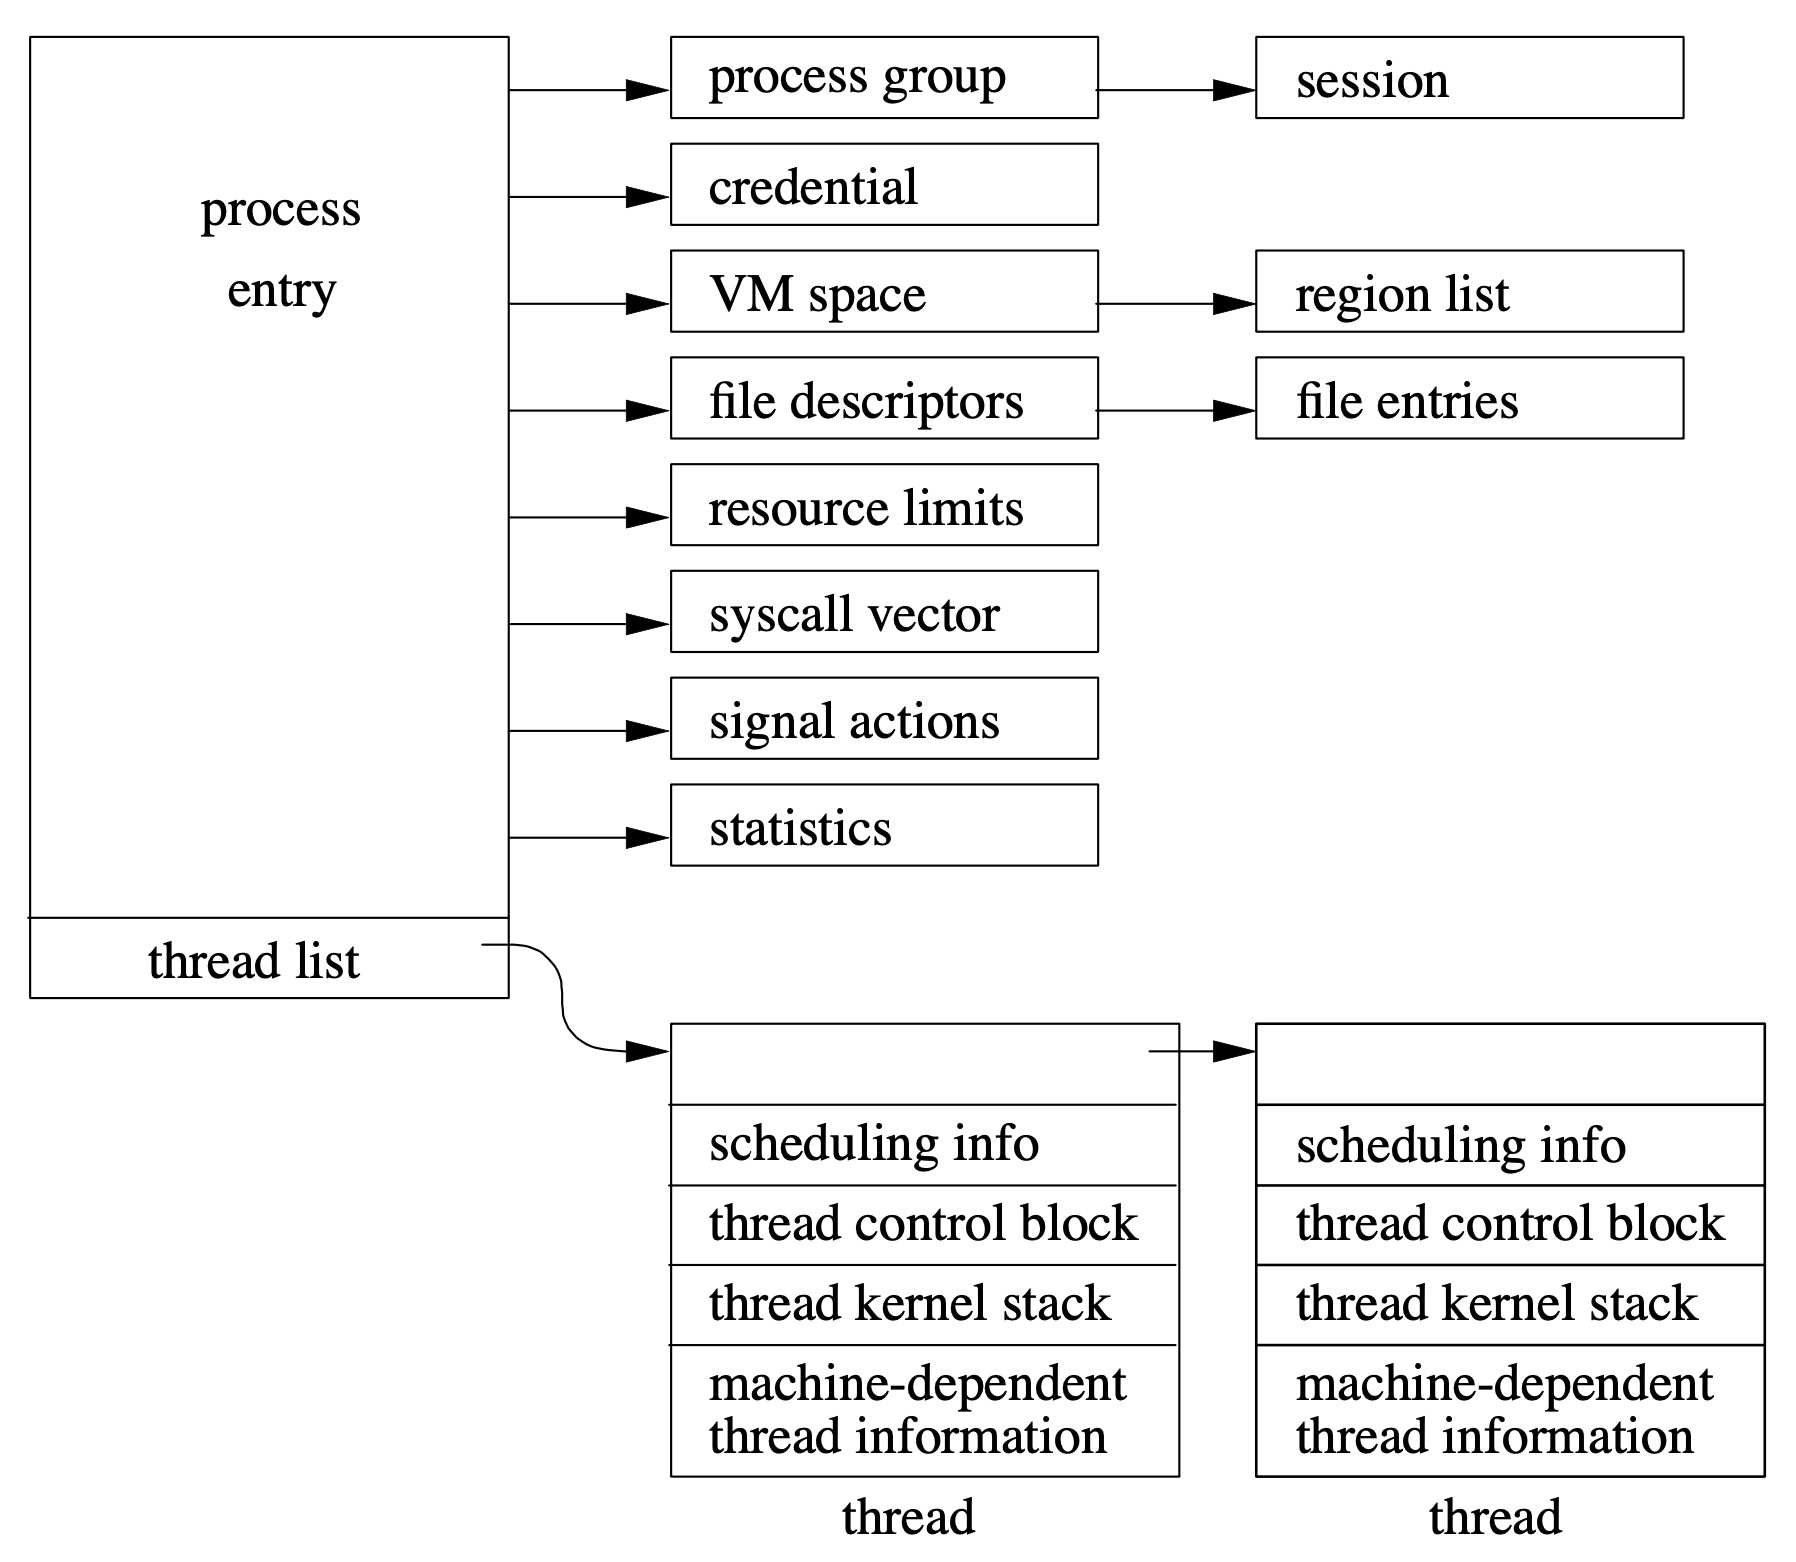
\includegraphics[width=0.6\textwidth]{images/processStructure.png}
    \caption{Estructura simplificada de un proceso.}
    \label{fig:process_state}
\end{figure}

\subsubsection{Estructura de hilos}
Un hilo, en el contexto de un proceso en un sistema operativo, es una entidad de ejecución que representa una secuencia independiente de instrucciones dentro de ese proceso. Cada hilo tiene su propio contador de programa, registros de CPU y pila de ejecución, lo que le permite ejecutar código de manera concurrente dentro del mismo proceso. Aunque los hilos comparten recursos como el espacio de direcciones y otros recursos del proceso principal, también pueden comunicarse y cooperar entre sí para llevar a cabo tareas específicas de manera más eficiente.\par

FreeBSD adopta el modelo 1:1, en el que cada hilo de usuario se corresponde con un hilo a nivel de kernel para mejorar la eficiencia de las aplicaciones.\par

La estructura de un hilo, que se muestra en la Figura \ref{fig:process_state}, solo contiene la información necesaria para ejecutarse en el kernel del sistema operativo:

\begin{itemize}
    \item Información para la planificación: se refiere a la prioridad del hilo en modo kernel y en modo usuario, la cantidad de tiempo que ha pasado suspendido y el uso reciente de la CPU. Además, se indica el estado de ejecución del hilo, banderas de estado adicionales; y si el hilo se encuentra suspendido, información sobre el canal y evento por el cual espera.
    \item TSB (thread state block): estado de ejecución del hilo en modo usuario y modo kernel. La estructura incluye registros de propósito general, punteros de pila, contador de programa, registros de gestión de memoria, entre otros.
    \item Pila del kernel: pila para usar al ejecutar en el kernel. Las pilas del kernel deben mantenerse pequeñas para evitar desperdiciar memoria física.
    \item Estado de la máquina (\textit{machine-dependent state}): se refiere a la información del hilo en relación a detalles que son específicos de la arquitectura de la CPU (registros de estado de punto flotante, información de interrupciones, información de registros de segmento de memoria, etc.).
\end{itemize}

\subsubsection{Estados de los procesos e hilos}

En FreeBSD, los procesos pueden encontrarse en uno de tres estados:

\begin{itemize}
    \item \uppercase{New}: Cuando se crea un proceso con la llamada al sistema fork.
    \item \uppercase{Normal}: El proceso pasa a este estado al asignarse suficientes recursos, permitiéndole comenzar su ejecución.
    \item \uppercase{Zombie}: Cuando un proceso ha completado su ejecución. En este estado, el proceso ha finalizado, pero aún no ha liberado todos sus recursos y no ha notificado su estado de finalización a su proceso padre.
\end{itemize}

El scheduler se encarga de planificar aquellos hilos correspondientes a procesos en estado NORMAL. Los hilos que conforman un proceso pueden encontrarse en diferentes estados:

\begin{itemize}
    \item \uppercase{inactive}: En proceso de creación y aún no han sido inicializados.
    \item \uppercase{inhibited}: Esperando por algún recurso del sistema o evento antes de poder ejecutarse.
    \item \uppercase{can\_run}: Inicializados y disponibles para ser agregados a alguna cola de ejecución.
    \item \uppercase{runq}: En la cola de ejecución, esperando su turno para ser ejecutados.
    \item \uppercase{running}: En ejecución.
\end{itemize}

\subsection{Planificación}

Planificar es decidir cómo, cuándo y por cuánto tiempo vamos a correr los hilos que se encuentran en nuestro sistema; tanto los hilos propios del sistema operativo, como de aplicaciones que se encuentran en ejecución.\par

En este sentido, la planificación es fundamental para equilibrar la utilización de los recursos con el tiempo necesario para completar los programas. FreeBSD implementa por defecto, un planificador \textit{compartido por tiempo}, el cual calcula la prioridad de los procesos de manera periódica. Este cálculo se realiza en base a datos previos, como la cantidad de tiempo utilizado de CPU o la cantidad de recursos de memoria que el proceso mantiene o requiere para su ejecución. No obstante, algunas tareas requieren un control más preciso sobre el proceso, como el caso de la planificación de tiempo real. FreeBSD también implementa esta funcionalidad mediante una cola separada para los hilos en cuestión, los cuales no se ven interrumpidos por otros hilos a menos que tengan igual o mayor prioridad.\par

Además, el \textit{kernel} de FreeBSD cuenta con una cola de hilos de mínima prioridad que se ejecutan únicamente cuando ningún otro hilo en las colas de mayor prioridad está en un estado de posible ejecución.\par

En cuanto al método de planificación por tiempo, FreeBSD favorece a los programas interactivos. Asigna una prioridad alta a cada hilo y permite que se ejecute por un periodo fijo de tiempo, conocido como \textit{time slice}. A medida que el hilo se ejecuta, su prioridad disminuye, mientras que aquellos suspendidos por E/S mantienen su prioridad. Por su parte, los hilos que se mantienen inactivos mejoran su prioridad en la cola.\par

\subsubsection{Elección del planificador}

La planificación a corto plazo en FreeBSD ha experimentado una notable evolución a lo largo de los años. Desde sus inicios con el planificador 4BSD hasta el actual planificador ULE, se han implementado cambios significativos que han contribuido a mejorar la eficiencia y el rendimiento del sistema.\par

Aunque el planificador ULE es el predeterminado en las versiones actuales de FreeBSD, este trabajo se basa en el trabajo previo realizado en el marco del proyecto integrador, que se centró en el planificador 4BSD\@. Para entender con mayor detalle y contexto dicha elección, visitar la sección 2.3.3.\ del proyecto integrador previo\cite{bib1}.

En este momento, nuestro enfoque principal no radica en realizar un cambio inmediato en el sistema operativo ni en contribuir directamente a la comunidad de FreeBSD\@. En su lugar, estamos continuando con la fase de investigación e implementación centrada en este tipo de planificadores.\par

Al mismo tiempo, el planificador 4BSD ha sido mantenido por la comunidad de FreeBSD durante décadas y no hay planes inmediatos para dejar de darle soporte. Esto significa que todavía sigue siendo una opción estable y confiable para el desarrollo de nuestro proyecto.\par

\subsubsection{Funcionamiento del planificador 4BSD}

El planificador 4BSD, inicialmente diseñado para sistemas monoprocesador, ha evolucionado para adaptarse eficazmente a sistemas multiprocesador. Comprender su funcionamiento es esencial para apreciar cómo este componente crítico del sistema FreeBSD gestiona la asignación de recursos y el tiempo de ejecución de los hilos.\par

En esencia, el planificador 4BSD organiza los hilos en múltiples colas según su prioridad. Cada hilo tiene una prioridad asignada y reside en una cola específica de acuerdo con esta prioridad.\par

Un aspecto crucial del planificador 4BSD es la gestión de tiempos de ejecución equitativos. A cada proceso se le asigna un pequeño período de tiempo, conocido como "timeslice". Una vez que un proceso agota su timeslice, se suspende temporalmente para permitir que otros procesos tengan la oportunidad de ejecutarse. Este proceso cíclico de asignación de tiempos de ejecución, basado en el algoritmo "Round Robin", asegura que ningún proceso monopolice los recursos del sistema durante largos períodos, contribuyendo así a un rendimiento estable y justo del sistema,  garantizando la equidad en el uso de los recursos del sistema.\par

En lo que respecta a las prioridades, el planificador 4BSD las ajusta periódicamente en función del tiempo de CPU consumido por cada hilo. Este proceso implica elevar la prioridad de los hilos que han utilizado menos tiempo de CPU y reducir la prioridad de aquellos que han consumido más recursos de procesador. De esta manera, el planificador se encarga de equilibrar la carga de trabajo de manera equitativa entre todos los procesos en ejecución en el sistema.\par

El rango de prioridades abarca desde 0 hasta 255, donde 0 denota la prioridad más alta. Las prioridades en el rango de 0 a 47 son asignadas de forma predeterminada por el sistema y se destinan a las tareas de interrupción.\par

Las prioridades de los hilos en tiempo real se encuentran en el intervalo de 48 a 79 y deben ser configuradas previamente por las aplicaciones mediante la llamada al sistema rtprio. A continuación, se encuentran los hilos con prioridades en el rango de 80 a 119, conocidos como hilos del kernel superior (top-half kernel threads). Estos hilos se encargan de gestionar operaciones críticas del kernel que afectan a todo el sistema.\par

Los hilos con prioridades entre 120 y 223 pertenecen a la clase de hilos de tiempo compartido o "user threads". Están destinados a ejecutar tareas de usuario convencionales y sus prioridades se ajustan de manera automática por el kernel en función del uso de la CPU.\par

Cuando no hay tareas activas que requieran el uso de la CPU, los hilos de la clase "IDLE" pueden ejecutarse. Estos hilos tienen la finalidad de mantener el sistema en un estado inactivo, consumiendo recursos mínimos y estando listos para responder a tareas prioritarias.\par

Adicionalmente, la Figura 2 ilustra de manera gráfica estas diferentes clases y rangos de prioridades para brindar una representación visual de cómo se distribuyen en el sistema.\par

\begin{table}[H]
    \centering
    \begin{tabular}{|c|c|c|}
        \hline
        \textbf{Rango} & \textbf{Clase} & \textbf{Tipo de hilo} \\
        \hline
        0 - 47 & ITHD & Bottom-half kernel (interrupt) \\
        \hline
        48 -79 & REALTIME & Real-time user \\
        \hline
        80 - 119 & KERN & Top-half kernel \\
        \hline
        120 - 223 & TIMESHARE & Time-sharing user \\
        \hline
        224 - 255 & IDLE & Idle user \\
        \hline
    \end{tabular}
    \caption{Clases de hilos por rango de prioridad.}
    \label{tabla:prio_hilos}
\end{table}

Esta representación gráfica ayuda a visualizar de manera clara la asignación de prioridades en el planificador 4BSD de FreeBSD.\par

\subsubsection{Encolado (add)}
El sistema usa 64 colas, seleccionando una cola para un determinado hilo y dividiendo la prioridad del hilo por 4. Para ahorrar tiempo, los hilos en cada cola no se vuelven a dividir en prioridades.\par

Estas colas pueden ser de tipo run queue, turnstile queue o sleep queue. Los hilos en estado RUNNABLE se ubican en las colas de tipo run queue; mientras que los que están bloqueados o esperando un evento, son posicionados en los otros dos tipos de colas.\par

Si un hilo agota su tiempo (o intervalo de tiempo) permitido, se coloca al final de la cola de la que procede, y el próximo hilo (ahora al principio de la cola) se selecciona para ejecutarse.\par

Si un hilo se bloquea, no se vuelve a colocar en la cola de ejecución (run queue). En su lugar, se coloca en una turnstile queue o en una sleep queue.\par

Las operaciones relacionadas al encolado se realizan dentro de la función sched\_add(). Ésta función recibe como parámetros el hilo a encolar y flags con información acerca del mismo.\par

Su primera tarea es corroborar que el hilo se encuentre en un estado permitido para ser encolado, es decir, en estado CAN\_RUN o RUNNING. Al pasar esta verificación, se adquiere el lock del planificador y se lo pasa al estado RUNQ para luego elegir en cuál cola de CPU va a ser asignado. Esto es posible a través de la función sched\_pickcpu(), la cual elige un CPU de la siguiente forma:

\begin{enumerate}
    \item Consulta si el hilo ya se había ejecutado en un procesador anterior y si es posible volverlo a encolar en el mismo. En caso de que sea verdadero, almacena este valor en una variable. En caso contrario, dentro de esa variable guarda el valor NOCPU (igual a -1).
    \item Luego itera a través de cada CPU disponible en el sistema. En caso de que el CPU que se está iterando no permita el encolado, continúa con el siguiente.
    \item Para el caso en que esté permitido el encolado para el CPU que se está iterando, existen dos opciones basadas en el valor de la variable inicializada en el primer punto.
    \begin{enumerate}
        \item En caso de que la variable haya sido inicializada con el valor NOCPU, se la sobreescribe con el CPU de la iteración en la que se encuentra el programa en ese momento.
        \item En caso de que la variable haya sido inicializada con el valor del último CPU en el que había sido ejecutado el hilo, se consulta si la cola del CPU que se está iterando, tiene menor cantidad de procesos que la del CPU elegido en el punto 1. Caso afirmativo, se reemplaza el valor de la variable por el CPU que se está iterando, ya que esto significa que éste procesador contiene menos hilos en su cola de ejecución. Caso contrario, el valor de la variable no se sobreescribe.
    \end{enumerate}
    \item Al finalizar la iteración de cada CPU, se retorna el valor de la variable con el CPU más apropiado para el hilo.
\end{enumerate}

Una vez elegido el mejor CPU para el hilo, se procede a realizar los cambios de contexto necesarios para agregarlo a la cola del procesador correspondiente.

Si el procesador al que se agrega el hilo es diferente al que está ejecutando la función en ese instante, éste último envía una señal IPI (inter-processor interrupt) para comunicar que existe este nuevo hilo en su cola.

En caso de que el hilo se agregara a la cola del CPU actual, se llama a las funciones correspondientes para saber si este hilo tiene mayor prioridad que el que está en ejecución actualmente y debe reemplazarlo, esto se conoce como preemption.

\subsubsection{Cambios de contexto (switch y throw)}
Al hablar de cambios de contexto de los hilos, se hace referencia a dos funciones en particular.\par

La función sched\_switch() se encarga de expulsar al hilo que recibe por parámetro (hilo actual en ejecución), o en caso de que el hilo continúe en estado RUNNING por alguna razón, se vuelve a poner en cola a través de la función sched\_add().\par

Una vez finalizada la expulsión se solicita un nuevo hilo para ejecutar. Esto se hace a través de la función choosethread() y sched\_choose().\par

Una vez obtenido el nuevo hilo, se verifica que éste no sea el mismo que fue puesto en cola anteriormente, si esto sucediera, sólo continúa la ejecución. Pero en caso de que sean dos hilos diferentes, se procede a realizar el cambio de contexto haciendo uso de la función cpu\_switch().\par

La función cpu\_switch() guarda el contexto del hilo anterior y restaura el contexto del nuevo hilo. Así como también, se asegura de que el estado del nuevo hilo se marque como TD\_RUNNING (en ejecución).\par

Otra de las funciones que se encargan del cambio de contexto es sched\_throw(), la cual se encarga de cambiar un hilo por otro en el mismo CPU que se está ejecutando. Recibe un hilo como parámetro (el cual puede ser nulo), y lo expulsa del planificador. Luego a través de la misma función utilizada anteriormente, choosethread(), obtiene un nuevo hilo y continúa con su ejecución.\par

\subsubsection{Elección de hilos (choose)}
La elección del próximo hilo a ejecutar se hace a través de la función sched\_choose() previamente invocada por la función choosethread() nombrada anteriormente.

El funcionamiento consiste en elegir al hilo con mayor prioridad dentro de alguna de las colas no vacías del CPU o de la cola global. Cada hilo habilitado para ser ejecutado, es decir en estado RUNNABLE, tiene una prioridad asignada.

La función comienza obteniendo el primer hilo de la cola global y el primero de la cola del CPU; guardando ambos en dos variables diferentes. Luego compara las prioridades de ambos y se queda con el de mayor prioridad.

Una vez elegido el hilo, se procede a removerlo de la cola correspondiente, ya sea la global o la del CPU, y se retorna este hilo.

Para el caso en que ambos hilos sean nulos, es decir, no hay hilos para ejecutar, se simula una ejecución con el idlethread y se retorna el mismo.

\subsubsection{Remoción de hilos de la cola (rem)}
A diferencia de la función anterior, en la que al elegir un hilo para correr, éste era removido de la cola en la que estaba ubicado, la función sched\_rem() se utiliza para quitar un hilo (especificado por parámetro) de una cola por dos razones principales.\par

Una de estas es el ajuste de prioridad que consiste en otorgarle una nueva prioridad al hilo por lo que es necesario removerlo de la cola en la que se encuentra y luego volver a encolarlo a través de la función sched\_add() en la posición correspondiente.\par

El otro motivo por el cual se querría hacer uso de esta función es en caso de que un hilo tenga afinidad con algún CPU, por lo que el procedimiento será igual al mencionado en el párrafo anterior, con el objetivo de que se encuentre en la cola correcta.\par

\subsection{Conceptos del proyecto integrador previo}

\subsubsection{Introducción}

El proyecto integrador del cual partimos, consiste en modelar el planificador 4BSD con Redes de Petri. Los hilos de ejecución de un proceso como el planificador del sistema operativo pueden considerarse como sistemas que pueden modelarse utilizando esta herramienta.\par

Las decisiones de encolado de los hilos en una CPU se toman a partir de la información representada en el modelo; así como también los estados globales y los de cada hilo.\par

\textcolor{red}{agregar alguito pa no pasar tan duracell}

\subsubsection{Modelado del hilo}
Uno de los modelos representados a través de la Red de Petri, es el de los estados de un hilo. En la figura es posible observar esta representación.\par

\textcolor{red}{Agregar red de petri del hilo}

\begin{itemize}
    \item \textbf{T0\_INIT}: El paso del estado INACTIVE a CAN\_RUN. Esto sucede cuando el hilo se agrega al planificador. Esto sucede generalmente en el momento de creación de un proceso o cuando el mismo realiza un fork. Esta tarea no corresponde al scheduler, por lo que inicialmente un hilo en el planificador se encuentra inicializado en el estado CAN\_RUN. Esta transición nunca se dispara, solo se la incorpora al modelo de modo representativo.
    \item \textbf{T1\_ON\_QUEUE}: El hilo se pone en una cola local de una determinada CPU o en la cola global dependiendo de la disponibilidad. Esta cola organiza los hilos de acuerdo a sus prioridades de ejecución.
    \item \textbf{T2\_SET\_RUNNING}: El hilo se quita de la cola y pasa a ejecutar las instrucciones del programa que tiene asignadas. En este instante el procesador se encuentra ocupado por dicho hilo.
    \item \textbf{T3\_SWITCH\_OUT}: El scheduler interrumpe el hilo y lo vuelve a colocar en una cola. El planificador toma otro hilo de la cola (el de mayor prioridad) y realiza un cambio de contexto.
    \item \textbf{T4\_TO\_WAIT\_CHANNEL}: Algún evento, semáforo o espera bloquea al hilo. Se agrega en una sleep queue o turnstile, en la cual el hilo queda a la espera de un evento que le quitará el bloqueo.
    \item \textbf{T5\_WAKEUP}: Se desbloquea el hilo y puede volver a encolarse nuevamente. El evento que lo desbloquea se genera fuera del scheduler. El hilo queda a la espera para poder cambiar de estado cuando corresponda.
    \item \textbf{T6\_REMOVE}: Se ejecutará cada vez que un hilo deba ser expulsado de la cola en que se encuentra actualmente.
\end{itemize}


\subsubsection{Modelado del planificador}

Para modelar el planificador se hace un modelo específico para un procesador y se extiende para los demás. En este proyecto se consideran cuatro procesadores.

\textcolor{red}{Agregar red de petri de 1 procesador}

Transiciones
\begin{itemize}
    \item TRAN\_ADDTOQUEUE: Un hilo es agregado a la cola del CPU correspondiente. Se encuentra inhibida cuando todo el sistema se encuentra en modo monoprocesador (al inicio del sistema operativo); y cuando ya existe un hilo en la cola.
    \item TRAN\_UNQUEUE: Se quita al hilo próximo a ejecutar de la cola del CPU. En este punto el hilo se encuentra listo para ser ejecutado.
    \item TRAN\_EXEC: El hilo pasa a ejecución por lo que el recurso del procesador se encuentra ocupado. Esta transición elimina el token de la plaza de habilitación, permitiendo así que un nuevo hilo pueda ser encolado. A su vez, ésta transición se encuentra inhibida en el modo monoprocesador.
    \item TRAN\_EXEC\_EMPTY: Esta transición se comporta de igual manera que la anterior, pero no depende de la plaza de habilitación. Su utilidad surge para los hilos provenientes de la cola global.
    \item TRAN\_RETURN\_VOL: Representa un retorno del recurso procesador para que pueda ejecutar otro hilo de su cola. Más precisamente, se dispara cuando la interrupción de la ejecución se debe a que el hilo no puede continuar porque espera por un evento o un recurso.
    \item TRAN\_RETURN\_INVOL: El funcionamiento es igual a la transición anterior, pero en este caso se dispara cuando la interrupción se produce porque el hilo consumió su tiempo asignado de CPU o bien finalizó su tarea.
    \item TRAN\_FROM\_GLOBAL\_CPU: Representa el desencolado de un hilo desde la cola global.
    \item TRAN\_REMOVE\_QUEUE: Expulsa un hilo de la cola y también resta un token de habilitación de la CPU, es decir, se premia a la misma para que pueda encolar.
    \item TRAN\_REMOVE\_EMPTY\_QUEUE: Su funcionamiento es igual al anterior pero se ejecuta en los casos en que la plaza de habilitación no posea ningún token.
    \item TRAN\_REMOVE\_GLOBAL\_QUEUE: Expulsa un hilo de la cola global. No premia al CPU.
    \item TRAN\_START\_SMP: Se dispara cuando el sistema pasa de monoprocesador a multiprocesador.
    \item TRAN\_THROW: Se ejecutará automáticamente cada vez que todas las plazas de habilitación de las CPU tengan al menos un token. El objetivo de esta transición consiste en habilitar las colas con la menor cantidad de hilos que estaban inhibidas, una vez que todas se han emparejado.
    \item TRAN\_QUEUE\_GLOBAL: Agrega un hilo a la cola global.
\end{itemize}


\subsubsection{Jerarquía de transiciones}
Para llevar a cabo la conexión entre las redes de los hilos y la red de recursos de las CPU se utiliza el concepto de redes jerárquicas. Es decir que al dispararse cierta transición en la red de recursos, también debe dispararse su transición correspondiente en la red del hilo.

Las jerarquías están definidas de la siguiente forma:
\begin{itemize}
    \item Transiciones TRAN\_ADDTOQUEUE y TRAN\_QUEUE\_GLOBAL de la red de recursos son jerárquicas a la transición T1\_ON\_QUEUE del hilo.
    \item Transiciones TRAN\_EXEC y TRAN\_EXEC\_EMPTY de la red de recursos son jerárquicas a la transición T2\_SET\_RUNNING del hilo.
    \item Transiciones TRAN\_REMOVE\_QUEUE, TRAN\_REMOVE\_EMPTY\_QUEUE y TRAN\_ REMOVE\_GLOBAL\_QUEUE de la red de recursos son jerárquicas a la transición T6\_ REMOVE del hilo.
    \item Transición TRAN\_RETURN\_INVOL de la red de recursos es jerárquica a la transición T3\_ SWITCH\_OUT del hilo.
    \item Transición TRAN\_RETURN\_VOL de la red de recursos es jerárquica a la transición T4\_TO \_WAIT\_CHANNEL del hilo.
\end{itemize}

\subsubsection{Marcado inicial}
La red de recursos se inicializará siempre con un token en la plaza que indica que el sistema se encuentra funcionando en modo monoprocesador. Además, se inicializan las plazas que representan a las CPU con un token, excepto la de la CPU0 ya que la misma, inicialmente se encuentra ejecutando el hilo inicial del sistema, por lo que esta última debe inicializarse con un token en la plaza de ejecución (PLACE\_EXECUTING\_0).

